\begin{figure}
\captionsetup[subfigure]{justification=centering}
\centering
\begin{tabular}{ccc}
\subcaptionbox{Belonging screen\label{fig:cross-device:fwvga37:belonging}}{ 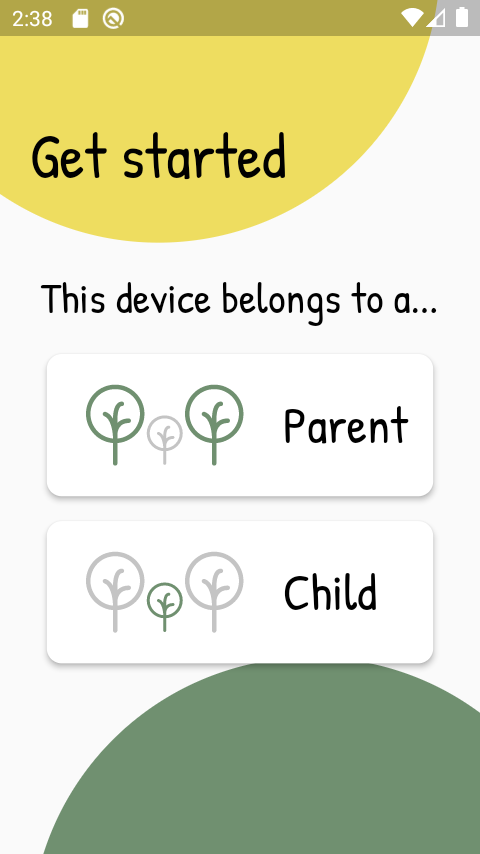
\includegraphics[width=.295\linewidth]{images/cross-device/FWVGA37/belonging.png}} 
&
\subcaptionbox{Login screen\label{fig:cross-device:fwvga37:login}}{ 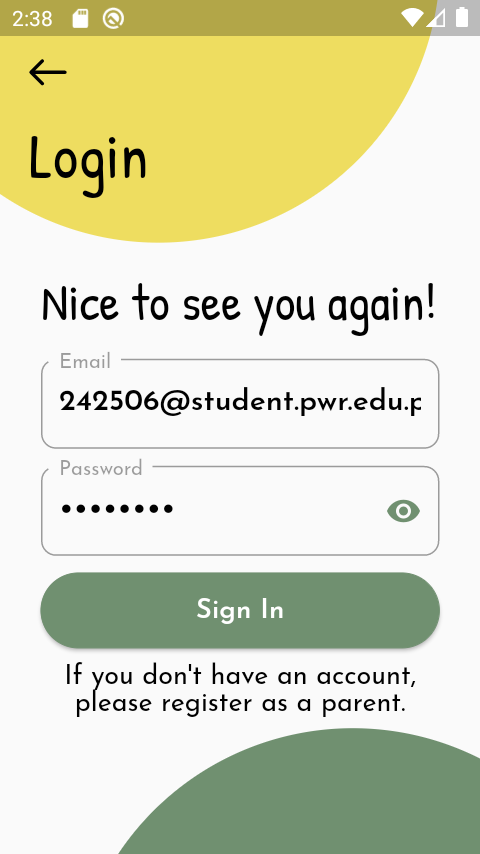
\includegraphics[width=.295\linewidth]{images/cross-device/FWVGA37/login.png}} 
&
\subcaptionbox{Children's profiles list screen\label{fig:cross-device:fwvga37:profiles}}{ 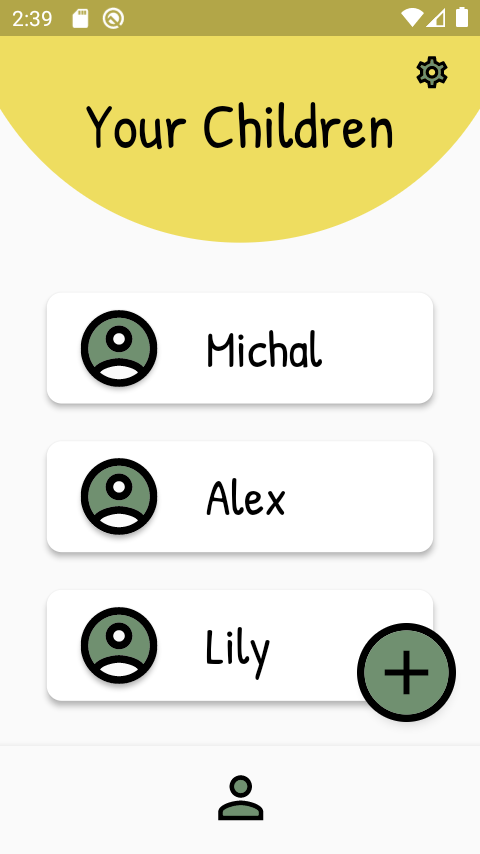
\includegraphics[width=.295\linewidth]{images/cross-device/FWVGA37/profiles.png}} 

\\\\\\\\
\subcaptionbox{Child's tasks screen\label{fig:cross-device:sgs6:tasks}}{ 
\includegraphics[width=.295\linewidth]{images/cross-device/FWVGA37/tasks.png}} 
&
\subcaptionbox{Task edit screen\label{fig:cross-device:fwvga37:edit-task}}{ 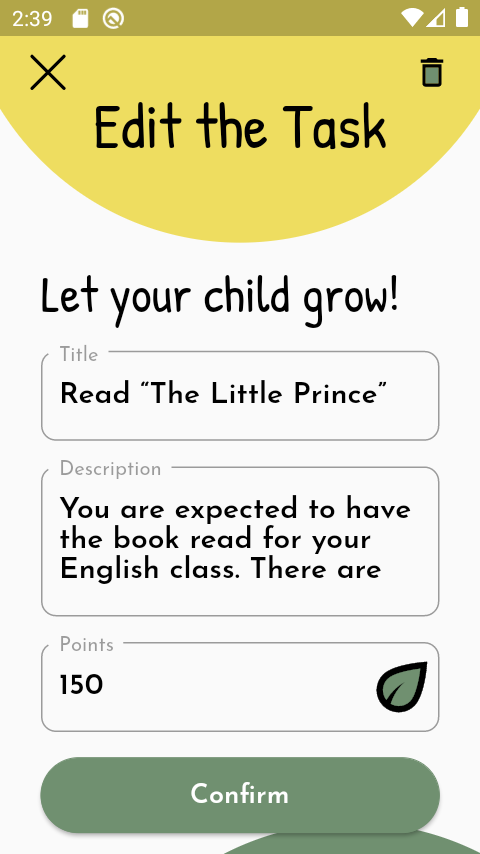
\includegraphics[width=.295\linewidth]{images/cross-device/FWVGA37/edit_task.png}} 
&
\subcaptionbox{Delete task confirmation\label{fig:cross-device:fwvga37:delete-task}}{ 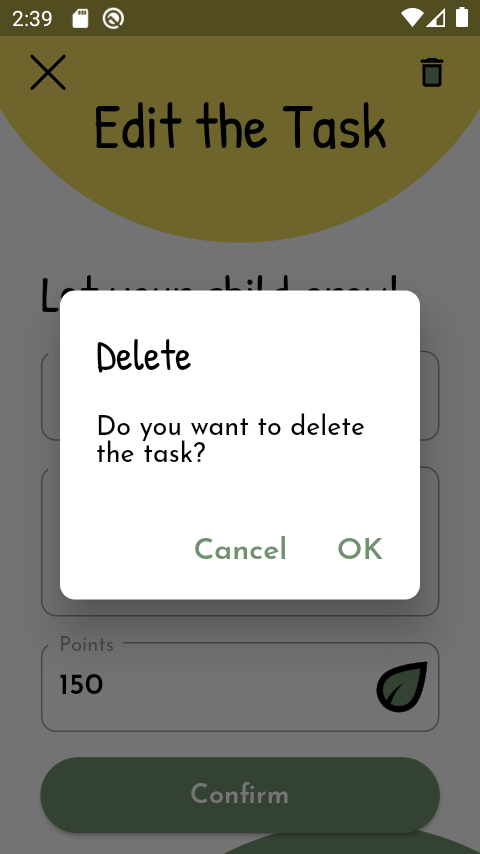
\includegraphics[width=.295\linewidth]{images/cross-device/FWVGA37/delete_task.png}} 
\end{tabular}
\caption{\textit{Raise App} selected screens displayed on the emulated device}
\label{fig:cross-device:fwvga37}
\end{figure}